\section{Allgemeinere Lineare Probleme}
\label{sec-4}

\subsection{Allgemeine Parameterabhängigkeit}
\label{sec-4.1}

Es folgt zunächst eine allgemeine Approximationsmethode für parametrische Funktionen, welche anschließend für RB-Behandlung von allgemeinen parametrisierten Problemen verwendet werden kann.

\subsubsection*{Empirische Interpolation (EI)}

\paragraph*{Motivation}

\begin{itemize}
	\item § \ref{sec-3} zeigte Relevanz der separierbaren Parameterabhängigkeit für effiziente Offline/Online-Zerlegung und Glattheit der Lösung $u(\mu)$ bzgl. $\mu$.
	\item Gesucht: Approximationsverfahren für parametrische Funktion
	\[
		g: \Omega \times \mathcal{P} \rightarrow \R
	\]
	der Form
	\[
		g(x;\mu) \approx I_{\mu} (g(\pdot;\mu))(x) = \sum\limits_{m=1}^M \Theta_g^m(\mu) g^m(x)
	\]
	mit skalaren Funktionen $\Theta_g^m(\mu)$ und ``kollaterale reduzierter Basis'' $Q_{\mu} = \{g^m\}_{m=1}^M$
	\item Statt allg. approx. Räume (z.\,B. FEM-Räume, zu hohe Dimension) oder Taylor-Ansatz (nur lokale Approx.) wird wieder Snapshot-basierter Ansatz gewählt, d.\,h. $Q_M \subset \op{span} \{g(\pdot,\mu)|_{\mu \in S_{train} \subset \mathcal{P}} \}$
	\item Die empirische Interpolation ist eine Mögllichkeit. Details finden sich in
	\begin{itemize}
		\item [BMNP04] Barrault, Maday, Nguyen, Patera: An ‘empirical interpolation’ method: application to efficient reduced-basis discretization of partial differential equations
		\item [MNPP07] Maday, Nguyen, Patera, Pau: A general, multipurpose interpolation procedure: the magic points
	\end{itemize}
\end{itemize}

\begin{defn}[Empirische Interpolation] \label{4.1}
	Sei $G \subset C^0(\bar{\Omega},\R)$ Menge von zu interpolierenden Funktionen. Für $\mu \in \N$, $M \leq \dim(\op{span}(G))$ definiere rekursiv Interpolationspunktemenge $T_{\mu} \subset \bar{\Omega}$ und die kollaterale Basis $Q_{\mu} \subset \op{span} (G)$
	\begin{align*}
	M = 1: \tilde{q}_1 &:= \op{argmax}_{g \in G} ||g||_{\infty} \\
	x_1 &:= \op{argmax}_{x \in \bar{\Omega}} |\tilde{q}_1 (x)| \\
	T_1 &:= \{x_1\} \\
	q_1 &:= \frac{\tilde{q}_1}{\tilde{q}_1 (x_1)} \\
	Q_1 &:= \{q_1\}
	\end{align*}
	\begin{align*}
	M > 1: \tilde{q}_M &:= \op{argmax}_{g \in G} ||g-I_{M-1}(g)||_{\infty} \\
	r_M &:= \tilde{q}_M - I_{M-1} \tilde{q}_M \\
	x_M &:= \op{argmax}_{x \in \bar{\Omega}} |r_M (x)| \\
	T_M &:= T_{M-1} \cup \{x_M\} \\
	q_M &:= \frac{r_M}{r_M (x_{\mu}} \\
	Q_M &:= Q_{M-1} \cup \{ q_M \}
	\end{align*}
	wobei $I_M : C^0(\bar{\Omega},\R) \rightarrow \op{span}(Q_{\mu})$ den Interpolationsparameter zu Punkten $T_M$ bezeichnet, d.\,h. $I_M(g)(x_i) = g(x_i) \,\, \forall \,\, g \in C^0(\bar{\Omega},\R)$, $i=1,\dots,M$.
\end{defn}

\begin{bem} \beginwithlistbem
	\begin{itemize}
		\item In der Praxis werden obige Optimierungsprobleme zur Bestimmung von $\tilde{q}_m$, $x_m$ durch einfache lineare Suche realisiert, indem endliche $\bar{\Omega}$ und $G$ betrachtet werden.
		\item Es sind Mehrdeutigkeiten von  $\tilde{q}_m$ und $x_m$ möglich, welche durch Aufzählung der Mengen und ``Wahl des ersten Auftretens'' eindeutig werden.
		\item Die Basis $Q_M$ ist weder orthogonal noch nodal, aber hierarchisch, d.\,h. $Q_{M-1} \subseteq Q_M$.
	\end{itemize}
\end{bem}

\begin{bem} \beginwithlistbem
	\begin{itemize}
		\item $Q_M$ sind beschränkt
		\[
			1 = q_m(x_m) = || q_m||_{\infty}
		\]
		Für analytische Untersuchungen wird später die nodale Basis $\zeta_M \subset \op{span} (Q_M)$ zu Knoten $T_M$ betrachtet, welche jedoch nicht mehr hierarchisch sind, d.\,h. $\zeta_{M-1} \not\subseteq \zeta_M$
		\item Die Erzeugung von $Q_M$ und $T_M$ kann als Greedy-Minimierungsstrategie  für
		
		 $\min\limits_{\substack{X_M \subset \op{span}(G) \\ \dim(X_M) = M \\ T_M \subset \bar{\Omega} \\ |T_M| = M}} \max\limits_{g \in G} ||g - I_M (g) ||_{\infty}$ interpretiert werden.
		
		Es kann jedoch kein monotoner Fehlerabfall garantiert werden.
	\end{itemize}
\end{bem}

\begin{satz}[Berechnung der Interpolation]
Seien $T_M = \{x_1,\dots,x_M\}$ und $Q_M = \{q_1,\dots,q_M\}$ gemäß Def. \ref{4.1} gegeben. Dann ist die Matrix $\underline{Q}_M := (\underline{q}_j(x_i))_{i,j=1}^M \in \R^{M \times M}$ eine untere Dreiecksmatrix mit 1-Diagonale, also regulär.
Sei $g \in C^0 (\bar{\Omega},\R), \underline{g}_M = (g(x_i))_{i=1}^M \in \R^M, \underline{\alpha}_M := (\alpha_i)_{i=1}^M \in \R^M$ Lösung von
\[
	\underline{Q}_M \underline{\alpha}_M = \underline{g}_M
\]
Dann ist die Interpolierte von $g$ gerade
\begin{align} \label{eq:4.1}
I_M (g) = \sum\limits_{i=1}^M \alpha_i \underline{q}_i
\end{align}
\begin{proof}
Seien $i,j = 1,\dots,M$
\begin{align*}
&i=j: (\underline{Q}_M)_{ii} = \underline{q}_i(x_i) = \frac{r_i(x_i)}{r_i(x_i)} = 1 \\
&j>i: (\underline{Q}_M)_{ij} = \underline{q}_j(x_i) = \frac{r_j(x_i)}{r_i(x_j)} = 0 \\
&\text{weil } r_j(x_i) = \underline{\tilde{q}}^{(x_i)} - I_{j-1}(\underline{\tilde{q}}_j)(x_i) = 0 \text{ da } I_{j-1} \text{ Interpolierende zu } T_{j-1} \text{ und } x_i \in T_{j-1}.
\end{align*}
Also $\underline{Q}_M$ untere Dreiecksmatrix mit 1-Diagonale.

Für \ref{eq:4.1} zeige Übereinstimmung von beiden Seiten in allen Interpolationspunkten $T_M$:

Für $i=1,\dots,M$ ist
\[
	\sum\limits_{j=1}^M \alpha_j \underline{q}_j(x_i) = \sum\limits_{j=1}^M \alpha_j (\underline{Q}_M)_{ij} = (\underline{Q}_M \underline{\alpha}_M)_i = (g_M)_i = g(x_i) = I_M(g)(x_i)
\]
\end{proof}
\end{satz}

\paragraph*{Beispiel (EI für Polynome)}
Sie $G= \{1,x,x^2\}$ Monome auf $\bar{\Omega} = [-1,1]$.
\begin{figure}[H]
  \centering\small
    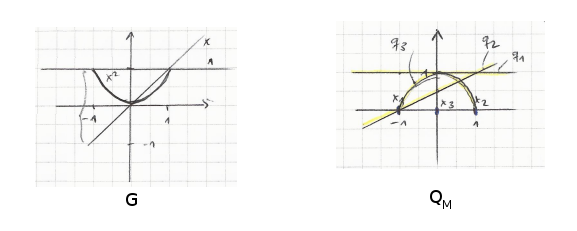
\includegraphics[width = 0.9 \textwidth]{Bilder/EI_Polynome.png}
  \label{fig:EI_Polynome}
\end{figure}
Dann ist
\[
	\underline{\tilde{q}}_1 := \op{argmax}\limits_{g \in G} ||g||_{\infty} \text{ beliebig, z.\,B. } \underline{\tilde{q}}_1(x) = 1
\]
und
\[
	x_1 = \op{argmax}_{x \in [-1,1]} |\underline{\tilde{q}}_1(x) \text{ beliebig, z.\,B. } x_1 = -1
\]
somit ergibt sich 
\[
\underline{q}_1(x) = \frac{\underline{\tilde{q}}_1(x)}{\underline{\tilde{q}}_1(x_1)} = 1
\]
Dann ist
\[
	\underline{\tilde{q}}_2 := \op{argmax}\limits_{g \in G} ||g - I_1(g)||_{\infty} = x,
\]
\[
	r_2 = \underline{\tilde{q}}_2 - I_1(\underline{\tilde{q}}_2) = x + 1,
\]
\[
	x_2 := \op{argmax}\limits_{x \in [-1,1]} |r_2(x)| = 1 \text{ und }
\]
\[
	\underline{q}_2(x) = \frac{r_2(x)}{r_2(x_2)} = \frac{1}{2} (x+1)
\]
schließlich
\[
	\underline{\tilde{q}}_3 := \op{argmax}\limits_{g \in G} ||g - I_2(g)||_{\infty} = x^2
\]
\[
	r_3 = x^2-1 \,\,\, , \,\,\, x_3 := \op{argmax}\limits_{x \in [-1,1]} |r_3(x)| = 0
\]
\[
	\underline{q}_3(x) = \frac{r_3(x)}{r_3(x_3)} = 1 - x^2
\]
\begin{center}
 \begin{tabular}{|c|c|c|c|c|}
 \hline
  $i$ & $x^i$ & $||x||_{\infty}$ & $||x^i - I_1(x^i)||_{\infty}$ & $||x^i - I_2(x^i)||_{\infty}$ \\ \hline
  $0$ & $1$ & $1$ & $||1-1||_{\infty} = 0$ & $0$ \\ \hline
  $1$ & $x$ & $1$ & $||x-(-1)||_{\infty} = 2$ & $0$ \\ \hline
  $2$ & $x^2$ & $1$ & $||x^2-1||_{\infty} = 1$ & $||x^2 - 1||_{\infty} = 1$ \\ \hline
 \end{tabular}
\end{center}

\paragraph*{Numerisches Beispiel} demos\_chapter4(1)

$G= \{x^i\}_{i=0}^{29}$

\begin{itemize}
 \item $\Rightarrow$ alle $q_i$ beschränkt, $||q_i||_{\infty} = 1$
 \item Fehler fällt nicht monoton
 \item $\cos^{-1}(T_M)$ ist etwa äquidistant, $T_M$ approximieren also qualitativ die Tschebyscheff-Knoten, die für polynomiale Interpolation als beste Wahl bekannt sind $\Rightarrow T_M$ sind sogennante ``Magic Points'' weil sie ``auf magische Weise'' wichtige Bereiche von $\Omega$ identifizieren.
\end{itemize}

\paragraph*{Eigenschafen der EI}

Wir untersuchen zunächst Stabilität der Interpolation. Dies geschieht durch Untersuchung der Lebesgue-Konstante (siehe Numerik I).

\begin{satz}[Lebesgue-Konstante]
Sie  $I_M:C^0(\Omega,\R) \rightarrow X_M := \op{span} (\zeta_i)_{i=1}^M \in C^0(\bar{\Omega},\R)$ Interpolationsoperator zu den Punkten $\{x_i\}_{i=1}^M$ und $\{\zeta\}_{i=1}^M$ nodal, d.\,h. $\zeta_i(x_j) = \delta_{ij}$, $I_M (u) = \sum\limits_{i=1}^M \zeta u(x_i)$. Dann ist
\[
	\Lambda_M := \max\limits_{x \in \bar{\Omega}} \sum\limits_{i=1}^M |\zeta_i (x)|
\]
die Lebesgue-Konstante der Interpolation.
\begin{enumerate}[i)]
	\item Es gilt
	\[
		|| u - I_M(u)||_{\infty} \leq (1 + \Lambda_M) \inf\limits_{v \in X_M} ||u-v||_{\infty}
	\]
	$\forall u \in C^0(\bar{\Omega},\R)$
	\item Für EI gilt
	\[
		\Lambda_M \leq 2^M -1
	\]
\end{enumerate}
\begin{proof}
\begin{enumerate}[i)]
	\item Sei $u \in C^0 (\bar{\Omega},\R), x \in \bar{\Omega}$ und $v = \sum a_i \zeta_i \in X_M$.
	
	Dann ist
\begin{align}	
	|u(x) - I_M(u)(x)| = |u(x) - \underbrace{\sum\limits_{i=1}^M a_i \zeta_i(x)}_{v(x)} + \underbrace{\sum\limits_{i=1}^M a_i \zeta_i(x)}_{v(x)} - \underbrace{\sum\limits_{i=1}^M u(x_i) \zeta_i(x)}_{I_M(u)(x)}| \notag \\ \leq |u(x) - v(x)| + |\sum\limits_{i=1}^M \zeta_i(x) \cdot (a_i - u(x_i))| \label{eq:4.2}
	\end{align}
	Für letzten Term gilt wegen $\{\zeta_i\}$ nodal
	\begin{align*}
	|\sum\limits_{i=1}^M \zeta_i(x) \cdot (a_i - u(x_i))| &= |\sum\limits_{i=1}^M \zeta_i(x) \cdot ((\underbrace{\sum\limits_{j=1}^M a_j \zeta_j(x_i))}_{a_i} - u(x_i))| \\
	&\leq \sum\limits_{i=1}^M |\zeta_i(x)| |v(x_i) - u(x_i)| \\
	&\leq \underbrace{(\max\limits_x \sum\limits_{i=1}^M |\zeta_i(x)|)}_{= \Lambda_M} \cdot ||u-v||_{\infty}
	\end{align*}
	Also für (\ref{eq:4.2}):
	\[
		||u-I_M(u)||_{\infty} \leq ||u-v||_{\infty} + \Lambda_M ||u-v||_{\infty} = (1 + \Lambda_M) ||u-v||_{\infty}
	\]
	nach Infimum über $v \in X_M$ folgt Behauptung.
	\item $\rightarrow$ Übung.
\end{enumerate}
\end{proof}
\end{satz}

\begin{bem} \beginwithlistbem
	\begin{itemize}
		\item Obige Abschätzung für $\Lambda_M$ ist sehr pessimistisch, in der Praxis meist bessere Raten/Lebesgue-Konstanten (langsameres Wachstum), jedoch ist die Schranke scharf, d.\,h. es ex. Beispiele mit $\Lambda_M = 2^M-1$.
		\item Für gewisse Mengen $G$ ist sogar exponentielle Konvergenz des Interpolationsfehleres beweisbar, wie in folgendem Satz. Dort auftretende Forderung ist ``Beschränktheit durch Müslipackung'', d.\,h. Polytop mit exponentiell abfallenden Seitenlängen.
	\end{itemize}
\end{bem}

\begin{satz}[Exponentielle Konvergenz der EI]
Falls es Sequenz von exponentiell approx. Unterräumen gibt, d.\,h. $Z_1 \subset Z_2 \subset \dots \subset Z_M \dots \subset \op{span}(G), \dim Z_M = M$ und ex. $c > 0, \alpha > \log 4$ so dass $\inf\limits_{v \in Z_M} ||u-v|| \leq c \cdot e^{-\alpha M} \,\,\, \forall \, u \in G, M \in \N$, dann findet der EI-Basiskonstruktionsprozess ``fast so gute Räume'' indem
\[
	||u-I_M(u)|| \leq c \cdot e^{-(\alpha - log 4)M}.
\]
\begin{proof}
	siehe MNPP07
\end{proof}
\end{satz}

Neben solchen a priori-Aussagen ist auch a posteriori-Fehlerkontrolle möglich.

\begin{satz}[A posteriori-Fehlerschätzer für EI] \label{4.5}
Seien $I_M, I_{M'}: C^0 (\bar{\Omega},\R) \rightarrow \op{span} (G)$ EI-Operatoren für $M' > M$, $Q_M \subset Q_{M'} = \{q_i\}_{i=1}^{M'}, T_M \subset T_{M'} = \{x_i\}_{i=1}^{M'}$.

Sei $\underline{Q} := (\underline{q}_i(x_i))_{i,j=M+1}^{M'}$. Für $g \in G$ sei $\underline{g} := (g(x_i)) - I_M(g)(x_i))_{i=M+1}^{M'}$ und $\underline{\alpha}' := \{\alpha_i '\}_{i=M+1}^{M'} := \underline{Q}^{-1} \underline{g}'.$

Falls $g \in \op{span}(Q_{M'}),$ so gelten folgende a posteriori-Fehlerschranken für den Interpolationsfehler:
\begin{align*}
||g-I_M(g)||_{\infty} &\leq \Delta_{M,M',\infty} (g) := ||\underline{\alpha}'||_1 = \sum\limits_{i=M+1}^{M'}|\alpha_i '| \\
||g-I_M(g)||_{L^2} &\leq \Delta_{M,M', L^2} (g) := \sqrt{(\underline{\alpha}')^T K_Q \underline{\alpha}'}
\end{align*}
mit $K_Q := (\int\limits_{\Omega} q_i q_j)_{i,j=M+1}^{M'}$
\begin{proof}
Nach Def. der EI gilt
\[
	I_M(g) = \sum\limits_{i=1}^M \alpha_i \underline{q}_i \,\, , \,\, I_{M'}(g) = \sum\limits_{i=1}^{M'} \alpha_i ' \underline{q}_i
\]
mit $\underline{Q}_M \underline{\alpha}_M = \underline{g}_M$ und $\underline{Q}_{M'} \underline{\alpha}_{M'} = \underline{g}_{M'}$
mit $\underline{\alpha}_M = (\alpha_i)_{i=1}^M, \underline{\alpha}_{M'} = (\alpha_i ')_{i=1}^{M'}$.

Da $\underline{Q}_M$ oberer linker Block von $\underline{Q}_{M'}$ und $\underline{Q}$ unterer rechter Block von $\underline{Q}_{M'}$, und jeweils untere Dreiecksmatrizen gilt $\alpha_i = \alpha_i '$, $i=1,\dots,M$ und $g-I_M(g) = I_{M'}(g) - I_M(g) = \sum\limits_{i=M+1}^{M'} \alpha_i ' \underline{q}_i$

Für $L^{\infty}$-Norm folgt $||g-I_M(g)||_{\infty} \leq \sum\limits_{i=M+1}^{M'} | \alpha_i ' | \underbrace{||\underline{q}_i||_{\infty}}_{1} = ||\underline{\alpha}'||_1$

Für $L^2$-Norm gilt $||g-I_M(g)||_{2} = \left(\sum\limits_{i,j=M+1}^{M'} \alpha_i ' \alpha_j ' \int\limits_{\bar{\Omega}} \underline{q}_i \underline{q}_j \right)^{\frac{1}{2}} = \Delta_{M,M',L^2}(g)$
\end{proof}
\end{satz}

\begin{satz}[Erhaltungseigenschaft]
Sie $f \in [C^0(\bar{\Omega},\R)]'$ und $f(g) = 0 \,\, \forall \, g \in G$.

Dann ist auch $f(I_M(g)) = 0 \,\, \forall \, g \in G$.
\begin{proof}
wg. Linearität folgt $f(\sum \beta_i g_i) = 0 \,\, \forall \, \beta_i \in \R, g_i \in G$
\[
	\Rightarrow f(g) = 0 \,\, \forall \, g \in \op{span}(G)
\]
Nach Konstruktion ist $Q_M \subseteq \op{span}(g)$, also $f(\underline{q}_i) = 0, i=1,\dots,M$, also auch $f(I_M(g)) = f(\sum \alpha_i \underline{q}_i) = 0 \,\, \forall \, g \in G$
\end{proof}
\end{satz}

\begin{bem} Anschauliche Beispiele
	\begin{itemize}
		\item[-] Falls $g(\bar{x}) = 0 \,\, \forall \, g \in G \Rightarrow I_M(g) (\bar{x})=0$ via $f \equiv$ Punktauswertung in $\bar{x}$.
		\item[-] Falls $g \in G$ haben Mittelwert $0$, d.\,h. $\int\limits_{\Omega} g(x) dx = 0 \,\, \forall \, g \in G$
		
		$\Rightarrow \int\limits_{\Omega} I_M(g) = 0 \,\, \forall \, g \in G.$
	\end{itemize}
\end{bem}

\paragraph*{Anwendung in RB-Methoden}
Falls eine Koeffizientenfunktion nicht separierbar parametrisch ist, erzeuge mittels EI eine separierbar parametrische Approximation.

\begin{defn}[EI für Funktionale]
Sie $f(v; \mu) = \int_{\Omega} g(x, \mu) v(x) dx$ parametrisch stetige Linearform, $g(\pdot; \mu) \in C^0 (\bar{\Omega},\R)$. Wähle $S_{train} \subset \mathcal{P}$ endliche Teilmenge, setze $G:= \{ g(\pdot;\mu) | \mu \in S_{train} \}$ Konstruiere EI-Basis $Q_M = \{q^i\}_{i=1}^M$ und EI-Punkte $T_M = \{x_i\}_{i=1}^M$ gemäß Definition \ref{4.1}. Dann ist $g(x;\mu) \approx \sum\limits_{m=1}^M \Theta^m(\mu)q^m(x)$ also
\[
	f(v;\mu) \approx \tilde{f}(v;\mu) := \sum\limits_{m=1}^M \Theta^m (\mu) \underbrace{\int\limits_{\Omega} q^m(x)v(x) dx}_{\tilde{f}^m(v)} =: \sum\limits_{m=1}^M \Theta^m(\mu) \tilde{f}^m(v)
\] 
Mit Komponenten $\{\tilde{f}^m\}_{m=1}^M$ und Koeffizienten $(\Theta^1(\mu), \dots, \Theta^m(\mu))^T := \underline{Q}_{M}^{-1} \underline{g}(\mu)$, wobei $\underline{g}\mu)$ durch lokale Auswertungen definiert ist
\[
	\underline{g}(\mu) = (g(x_1;\mu),\dots,g(x_M;\mu))^T
\]
\end{defn}

\begin{bem} \beginwithlistbem
	\begin{itemize}
		\item Analoge Vorgehensweise bei Ausgabefunktional oder Bilinearform möglich. Anschließend Offline/Online Zerlegung wie in §\ref{sec-3} realisierbar.
		\item Fehlerschätzer aus §\ref{sec-3} sind mit EI  im Allgemeinen nicht rigoros, da der Interpolationsfehler zusätzlich berücksichtigt werden muss. Falls $g(\pdot;\mu) \in \op{span} (Q_M)$ (starke Annahme) so sind Schätzer weiterhin rigoros.
		\item Falls Interpolatinosfehler $\neq 0$, aber Fehlerschätzer für EI vorhanden, so kann mittels eines Hilfsproblems (hochdimensionales interpoliertes Problem) $(\tilde{\mathcal{P}}(\mu))$ Fehlerkontrolle für das interpolierte und reduzierte Problem realisiert werden. (wir ignorieren wieder Ausgabe im Folgenden).
	\end{itemize}
\end{bem}

\begin{defn}[Interpolierte Probleme $(\tilde{P}(\mu))$, $(\tilde{P}_N(\mu))$] \label{4.8}
Sei eine Instanz von $(P(\mu))$ gegeben mit $a(\pdot,\pdot;\mu)$ koerziv. Seien Approximationen $\tilde{a}(\pdot,\pdot;\mu)$ und $\tilde{f}(\pdot;\mu)$ bilinear/linear gegeben mit $\tilde{a}$, $\tilde{f}$ separierbar parametrisch und
\begin{align*}
	| a(u,v;\mu) - \tilde{a}(u,v;\mu) | &\leq \epsilon_a ||u|| ||v|| &\forall u,v \in X, \mu \in \mathcal{P} \\
	|f(v;\mu) - \tilde{f}(v;\mu) | &\leq \epsilon_f ||v|| &\forall v \in X, \mu \in \mathcal{P}
\end{align*} 
mit möglichen kleinen Approximationsfehlern $\epsilon_a$, $\epsilon_f \geq 0$.

Wir nennen $\tilde{u}(\mu) \in X$ Lösung des \emph{vollen interpolierten Problems} $(\tilde{P}(\mu))$
\[
	\tilde{a}(\tilde{u}(\mu),v;\mu) = \tilde{f}(v;\mu)	\qquad \forall v \in X
\]
und $\tilde{u}_N \in X_N$ Lösung des \emph{reduzierten interpolierten Problems} $(\tilde{P}_N(\mu))$
\[
	\tilde{a}(\tilde{u}_N(\mu),v;\mu) = \tilde{f}(v;\mu)	\qquad \forall v \in X_N
\]
für beliebige gewählten $X_N \subset X$.
\end{defn}

\begin{bem}[Beispiele für $\epsilon_a$, $\epsilon_f$, aus EI]
Sie $X=H_0^1(\Omega)$ und $f(v) = \int_{\Omega} q(x) v(x) dx$ mit $q \in L^1(\Omega) \cap C^0(\Omega)$ und $q_M$ EI von $q$, damit $\tilde{f}(v) := \int_{\Omega} q_M(x)v(x) dx$
\begin{align*}
& \Rightarrow |f(v) - \tilde{f}(v)| = | \int_{\Omega} (q(x) - q_M(x)) v(x) dx | \overset{CS}{\leq} || q - q_M||_{L^2} \underbrace{||v||_{L^2}}_{\leq ||v||_{H_0^1}} \overset{\ref{4.5}}{\leq} \Delta_{\mu;\mu;2} (q) ||v|| \\
& \Rightarrow \epsilon_f := \Delta_{\mu;\mu;2} (q) \text{ (bzw. Supremum über } \mathcal{P} \text{ falls } q \text{ parametrisch)}
\end{align*}
Sei z.\,B. $a(u,v) = \int_{\Omega} \kappa(x;\mu) u(x) v(x) dx$ mit $\kappa(x;\mu) \in C^0(\bar{\Omega})$ und $\kappa_{\mu}$ EI von $\kappa$
\[
	\tilde{a}(u,v) = \int_{\Omega} \kappa_{\mu} (x;\mu) u(x) v(x) dx
\]
\begin{align*}
	& \Rightarrow |a(u,v) - \tilde{a}(u,v) | \leq || \kappa - \kappa_{\mu}||_{\infty} \underbrace{|\int_{\Omega} u(x) v(x) dx|}_{\leq ||u||_{L^2} ||v||_{L^2}} \leq || u||_{H_0^1} ||v||_{H_0^1} \Delta_{\mu;\mu;\infty} (\kappa) \\
	& \Rightarrow \epsilon_a := \sup\limits_{\mu \in \mathcal{P}} \Delta_{\mu;\mu;\infty} (\kappa(\pdot;\mu))
\end{align*}
\end{bem}

\begin{bem}[Wohlgestelltheit von $(\tilde{P}(\mu))$, $(\tilde{P}_N(\mu))$]
Falls $\epsilon_a$, $\epsilon_f$ genügend klein, sind $\tilde{a}$, $\tilde{f}$ stetig, $\tilde{a}$ ist koerziv, damit ist $(\tilde{P}(\mu))$ nach Lax-Milgram wohlgestellt (Existenz \& Eindeutigkeit \& Stabilität bzgl. rechter Seite). Genauer: Bei $\epsilon_a$, $\epsilon_f < \infty$ folgt Stetigkeit.
\begin{align*}
 &|\tilde{f}(v)| \leq |\tilde{f}(v) - f(v) | + |f(v)| \leq \epsilon_f ||v|| + ||f|| \cdot ||v|| = (\epsilon_f + ||f||_{X'}) ||v|| \\
 \Rightarrow &\tilde{f} \in X' \text{ mit } ||\tilde{f}|| \leq ||f|| + \epsilon_f
\end{align*}
Falls $\epsilon_a < \alpha$ mit $\alpha$ Koerzivitätskonstante von $a(\pdot,\pdot)$, so folgt
\[
	\frac{\tilde{a}(u,u)}{||u||^2} = \frac{a(u,u)-(a(u,u) - \tilde{a}(u,u))}{||u||^2} \geq \underbrace{\frac{a(u,u)}{||u||^2}}_{\geq \alpha} - \underbrace{\frac{|\tilde{a}(u,u)|}{||u||^2}}_{\leq \epsilon_a} \geq \alpha - \epsilon_a > 0
\]
also $\tilde{a}$ koerziv mit Koerzivitätskonstante $\tilde{\alpha} \geq \alpha - \epsilon_a$.
\end{bem}

\begin{bem}[Schranke $||u - \tilde{u}||$]
Falls $\epsilon_a < \alpha$ so folgt mit Störungsargument eine Schranke für $||u - \tilde{u}||$ bezüglich $\epsilon_a$, $\epsilon_f$
\[
	a(u - \tilde{u},v) = a(u,v) - a(\tilde{u},v) = f(v) - a(\tilde{u},v) =: r(v, \tilde{u})
\]
Lax-Milgram liefert also mit $r(v,\tilde{u}) = f(v) - \underbrace{\tilde{f}(v) + a(\tilde{u},v)}_{0} - a(\tilde{u},v)$.
\begin{align} \label{eq:4.2}
 || u- \tilde{u}|| \leq \frac{|||r(\pdot;\tilde{u})||_{X'}}{\alpha} \leq \frac{1}{\alpha} (\epsilon_f + \epsilon_a ||\tilde{u}||)
\end{align}
Für $||\tilde{u}||$ liefert Lax-Milgram
\[
	||\tilde{u}|| \leq \frac{||\tilde{f}||}{\tilde{\alpha}} \leq \frac{||\tilde{f}||}{\alpha - \epsilon_a}
\]
also insgesamt in \ref{eq:4.2}
\begin{align} \label{eq:4.3}
	|| u - \tilde{u}|| \leq \frac{1}{\alpha} \epsilon_f + \frac{||\tilde{f}||}{\alpha(\alpha - \epsilon_a)} \epsilon_a =: \Delta_{EI}
\end{align}
Dreiecksungleichung $||u-\tilde{u}_N|| \leq || u - \tilde{u}|| + ||\tilde{u} - \tilde{u}_N||$ und deren Schranken (\ref{eq:4.3}) bzw. $\Delta_N$ liefern:
\end{bem}

\begin{kor}[EI-RB Fehlerschranke]
Seien $(P(\mu))$, $(\tilde{P}(\mu))$, $(\tilde{P}_N(\mu))$ wie in Definition \ref{4.8} gegeben und $\epsilon_a < \alpha$ Dann gilt die Fehlerschranke
\[
	||u(\mu) - u_N(\mu) || \leq \Delta_{EI} (\mu) + \Delta_N (\mu)
\]
mit $\Delta_{EI} (\mu)$ aus (\ref{eq:4.3}) und $\Delta_N(\mu)$ Standard RB-Fehlerschranke für $||\tilde{u} - \tilde{u}_N||$ aus Satz \ref{3.13} ii).
\end{kor}

\subsection{Inf-sup stabile Probleme}

\begin{defn}[inf-sup Stabilität]
Eine stetige Bilineaform $a: X_1 \times X_2 \rightarrow \R$ heißt \emph{inf-sup stabil} auf $X_1 \times X_2$ mit \emph{inf-sup-Konstante} $\beta$ falls
\[
	\beta := \inf\limits_{v \in X_1 \backslash \{0\}} \sup\limits_{w \in X_2 \backslash \{0\}} \frac{a(v,w)}{||v|| ||w||} > 0
\]
Wir fassen einige Einsichten/Aussagen zu inf-sup stabilen Problemen zusammen, für Beweise siehe Skript NUMPD14/15 oder Braess FEM.
\end{defn}

\begin{bem}[Beziehung zwischen $\alpha$/$\beta$] \beginwithlistbem
\begin{itemize}
	\item inf-sup Stabilität ist allgemeinerer Stabilitätsbegriff als Koerzivität.
	
	falls $a$ koerziv $\Rightarrow$ $a$ inf-sup stabil mit $\beta \geq \alpha$
	
	falls $a$ koerziv \& symmetrisch $\Rightarrow$ $a$ inf-sup stabil mit $\beta = \alpha$
	
	$\beta$ ist also immer ``bessere'' (oder gleich gute) Konstante als $\alpha$.
	\item inf-sup Stabilität vererbt sich nicht auf Teilräume dies stellt bei FEM- und RB-Behandlung ein Problem dar.
\end{itemize}
\end{bem}

\begin{bem}[Beispiel] \beginwithlistbem
\begin{enumerate}[a)]
\item Divergenzgleichung:  Sie $\Omega$ Lipschitz-Gebiet und beschränkt

Für $q \in Q_1 := L_0^2(\Omega) = \{p \in L^2 (\Omega) | \int_{\Omega} p(x) dx = 0 \}$ und $v \in V := H_0^1(\Omega)^d$ ist $a(q,v) = \int_{\Omega} q \op{div}(v)$ inf-sup stabil auf $Q \times V$.
\item Stokes-Problem:
\[
	-\mu \Delta u + \nabla p = r \qquad \text{ in } \Omega, \,\,\, \op{div} u=0 \, \text{ in } \Omega, \,\,\, u= 0 \, \text{ auf } \Gamma
\]
ergibt mit $X_1 := X_2 := H_0^1(\Omega)^d \times L_0^2(\Omega)$ schwache Form:

Suche $(u,p) \in X_1$ so dass $a((u,p),(v,q)) = f((v,q)) \qquad \forall (v,q) \in X_2$ 

mit $a((u,p),(v,q)) := \mu \int_{\Omega} \nabla u : \nabla v - \int_{\Omega} p \op{div}(v) - \int_{\Omega} q \op{div}(u)$.

Dann ist $a$ inf-sup stabil auf $X_1 \times X_2$.
\end{enumerate}
Der folgende Satz garantiert Wohlgestelltheit für inf-sup stabile Probleme
\end{bem}

\begin{satz}[Ne\v{c}as-Theorem] \label{4.11}
Sei $a: X_1 \times X_2$ stetig Bilinearform, $l \in X'_2$. Die Gleichung
\[
	a(u,v) = l(v) \qquad \forall v \in X_2
\]
hat eine eindeutige Lösung $u \in X_1$ und ist stetig von den Daten abhängig via
\[
	||u||_{X_1} \leq \frac{1}{\beta} ||l||_{X'_2}
\]
für ein $\beta > 0$ (unabhängig von $l$) genau dann wenn eine der folgenden Bedingungen gilt:
\begin{enumerate}[i)]
	\item $a(\pdot,\pdot)$ erfüllt $\inf\limits_v \sup\limits_w \frac{a(v,w)}{||v||_{X_1} ||w||_{X_2}} \geq \beta > 0$
	
	und $\forall w \in X_2$, $w \neq 0$ ex. $v \in X_1$ mit $a(v,w) \neq 0$.
	\item $a(\pdot,\pdot)$ erfüllt $\inf\limits_w \sup\limits_v \frac{a(v,w)}{||v||_{X_1} ||w||_{X_2}} \geq \beta > 0$
	
	und $\forall v \in X_1$, $v \neq 0$ ex. $w \in X_2$ mit $a(v,w) \neq 0$.
\end{enumerate}
\begin{proof}
	z.\,B. Satz 3.57 in NUMPDE14/15
\end{proof}
\end{satz}

\begin{bem} \beginwithlistbem
\begin{itemize}
	\item inf-sup Stabilität ist also ``allgemeinerer'' Stabilitätsbegriff, welcher Wohlgestelltheit impliziert.
	\item Lax-Milgram kann als Korollar von \ref{4.11} gezeigt werden
	\item Aus \ref{4.11} folgt insbesondere
	\begin{align} \label{eq:4.4}
		\text{wohlgestellt} \Rightarrow \inf\limits_{v \in X_1} \sup\limits_{w \in X_2} \frac{a(v,w)}{||v|| ||w||} = \beta = \inf\limits_{w \in X_2} \sup\limits_{v \in X_1} \frac{a(v,w)}{||v|| ||w||}
	\end{align}
	also dasselbe $\beta$ für beide Richtungen. Umgekehrte Richtung in (\ref{eq:4.4}) gilt auch.
\end{itemize}
\end{bem}

\begin{satz}[Eigenschaften von $\beta$/ Suprimierender Operator] \label{4.12}
Sie $a(\pdot,\pdot)$ stetige Bilinearform auf $X_1 \times X_2$ und
\[
	a(u,v) = \dotp{Au}{v}_{X_2} \qquad \forall (u,v) \in X_1 \times X_2
\]
mit Operator $A \in L(X_1,X_2)$. Dann gilt:
\begin{enumerate}[i)]
	\item $A$ ist \emph{suprimierender Operator},
	\[
		\sup\limits_{v \in X_2} \frac{a(u,v)}{||v||} = \frac{a(u,Au)}{||Au||} \qquad \forall u \in X_1 \backslash \{0\}
	\]
	\item \[
		\beta = \inf\limits_{u \neq 0} \frac{||Au||}{||u||}
	\]
	\item \[
		\gamma = \sup\limits_{u \neq 0} \frac{||Au||}{||u||}
	\]
	\item $\forall u \in X_1$ ex. $v \in X_2$ s.\,d. $\beta ||u|| ||v|| \leq a(u,v)$
	\item $A$ ist injektiv, d.\,h. $\forall v \neq 0$ gilt $Av \neq 0$.
\end{enumerate}
\begin{proof}
	Satz 3.32 in NUMPDE14/15
\end{proof}
\end{satz}

\begin{bem}
Solches $A$ existiert wegen Riesz: $a(u,\pdot) \in X'_2$ also existiert Riesz-Repräsentant $Au \in X_2$ mit $a(u,\pdot) = \dotp{Au}{\pdot}_{X_2}$.
\end{bem}

\begin{satz}[Eigenwert für $\beta$/$\gamma$] \label{4.13}
Seien $X_1$, $X_2$ Hilberträume, $a: X_1 \times X_2$ stetige Bilinearform mit $a(u,v) = \dotp{Au}{v}$ und $A$, $A^*$ komp. Operator d.h. $A \in K(X_1,X_2)$, $A^* \in L(X_2,X_1)$ und $\sigma := \sigma(A^*A)$ Spektrum von $A^*A$. Dann gilt:
\begin{enumerate}[i)]
	\item $\forall \lambda \in \sigma$ ex. $u \in X_1$:
	\[
		\dotp{Au}{Av}_{X_2} = \lambda \dotp{u}{v}_{X_1} \qquad \forall v \in X_1
	\]
	\item $\beta^2 = \inf \sigma$
	\item $\gamma^2 = \max \sigma$
\end{enumerate}
\begin{proof}
\begin{enumerate}[i)]
\item Seien $u, \lambda$ EV/EW von $A^*A$ $\Rightarrow \dotp{A^*Au}{v}_{X_1} = \dotp{\lambda u}{v}_{X_1} \qquad \forall v \in X_1$
\[
	\Rightarrow \dotp{Au}{Av}_{X_1} = \lambda \dotp{u}{v}_{X_1} \qquad \forall v \in X_1
\]
\item Wegen $A^*A$ komp. \& selbstadjungiert folgt mit Spektralsatz
\[
	A^*Au = \sum\limits_{i \in I} \lambda_i \dotp{u}{\phi_i}\phi_i
\]
und $\sigma = \{\lambda_i\}_{i \in I}$ oder $\sigma = \{\lambda_i\}_{i \in I} \cup \{0\}$

Nach \ref{4.12} ii) $\beta = \inf\limits_{u \neq 0} \frac{||Au||}{||u||} = \inf\limits_{u \neq 0} \sqrt{\frac{||Au||^2}{||u||^2}} = \inf\limits_{||u|| = 1} \sqrt{\dotp{Au}{Au}} = \inf\limits_{||u||=1} \sqrt{\dotp{A^*Au}{A}}$
\begin{align} \label{eq:4.4}
\beta^2 = \inf\limits_{||u||=1} \dotp{A^*Au}{u}
\end{align}
Falls $0 \in \sigma$ mit EV $\phi^0 \Rightarrow 0 \leq \beta^2 = \dotp{A^*A\phi^0}{\phi^0} = 0 \Rightarrow \beta^2 = 0 = \inf \sigma$.

Falls $0 \not\in \sigma \Rightarrow \{\phi_i\}_{i \in I}$ ist vollständiges ONS von $X_1$
\begin{align*}
	&\Rightarrow \forall u \in X_1 \text{ mit } ||u||=1 \text{ ex. } u_i \in \R \text{ mit } u = \sum\limits_{i \in I} u_i \phi_i \, , \, \sum u_i^2 = 1 \\
	&\overset{(\ref{eq:4.4})}{\Rightarrow} \beta = \inf\limits_{||u||=1} \dotp{A^*Au}{u} = \inf\limits_{||u||=1} \sum \lambda_i u_i^2  \underbrace{\geq}_{\text{Konvexkombination}} \inf \{\lambda_i\} = \inf \sigma
\end{align*}
und $\beta^2 = \inf\limits_{||u||=1} \sum \lambda_i u_i^2 \underbrace{\leq}_{u = \phi_j} \sum \lambda_i u_i^2 = \lambda_j \Rightarrow \beta^2 \leq \inf \{\lambda_i\} \Rightarrow \beta^2 = \inf \sigma$
\item analog zu ii)
\end{enumerate}
\end{proof}
\end{satz}

\begin{kor}[Inf-sup Stabilität im Endlichdimensionalen]
Sei $X_1 = \R^m, X_2 = \R^n, A \in \R^{n \times m}$, $m \leq n$ und $a(u,v) := \dotp{Au}{v}$. Seien $\{\sigma_i\}_{i=1}^m$ Singulärwerte von $A$. Dann
\begin{enumerate}[i)]
	\item $\beta = \min\limits_{i=1,\dots,m} \sigma_i$
	\item $a$ inf-sup stabil $\iff$ $A$ hat vollen Spaltenrang
\end{enumerate}
\begin{proof}
\begin{enumerate}[i)]
	\item $a$ stetig und $A, A^T$ kompakter linearer Operator, da endlichdimensionale  Bilder. Mit \ref{4.13} folgt wegen $\sigma(A^TA) = \{\sigma_i^2\}_{i=1}^m : \beta^2 = \inf \sigma(A^TA) = \min\limits_{i=1,\dots,m} \{\sigma_i^2\}$. Weil $\beta \geq 0, \sigma_i \geq 2 \Rightarrow \beta = \min\limits_{i=1,\dots,m} (\sigma_i)$.
	\item $a$ inf-sup-stabil $\iff \beta > 0 \overset{i)}{\iff} \sigma_i > 0 \,\, \forall \, i \iff A \text{ hat Rang } m \iff \text{ A hat vollen Spaltenrang.}$
\end{enumerate}
\end{proof}
\end{kor}

RB-Methode folgt mit \emph{Petrov Galerkin-Projektion}

\begin{defn}[$(P(\mu)), (P_N(\mu))$ für inf-sup stabilen Fall] \label{4.15}
Sei $a: X_1 \times X_2 \times \mathcal{P} \rightarrow \R$ stetig param. Bilinearform, $a(\pdot,\pdot;\mu)$ inf-sup stabil mit $\beta(\mu)$ inf-sup Konstante $f(\pdot;\mu)$ stetig param. Linearform. Zu $\mu \in \mathcal{P}$ ist $u(ßmu) \in X_1$ Lösung des vollen Problems
\[
	a(u(\mu),v;\mu) = f(v;\mu) \qquad \forall \,\, v \in X_2
\]
Seien $X_{N,1} \subseteq X_1$, $X_{N,2} \subseteq X_2$ mit $N = \dim X_{N,1} = \dim X_{N,2}$ RB-Räume. Dann ist $u_N (\mu) \in X_{N,1}$ RB-Lösung von
\[
	a(u_N(\mu),v;\mu) = f(v;\mu) \qquad \forall \,\, v \in X_{N,2}
\]
\end{defn}

\begin{bem} \beginwithlistbem
	\begin{itemize}
		\item Wir verzichten in \ref{4.15} auf das Ausgabefunktional, dies kann analog zu §\ref{sec-3.5} behandelt werden, d.\,h. $l$ parametrische Linearform
		\begin{align}
			&s'_N(\mu) = l(u_N(\mu);\mu) - r(u_N^{du};\mu) \text{ mit } u_N^{du} \in X_{N,2}^{du} \text{ Lösung von} \label{eq:4.5} \\
			&a(v, u_N^{du};\mu) = -l(v;\mu) \,\, \forall \,\, v \in X_{N,1}^{du} \text{ und dualen RB-Räumen } X_{N,1}^{du}, X_{N,2}^{du} \label{eq:4.6}
		\end{align}
		\item Wahl von $X_{N,1}, X_{N,2}$ ist nicht beliebig, sondern müssen geeignet gewählt werden, so dass $(P_N(\mu))$ gute Approximation liefert (wie in §\ref{sec-3}. Wähle $X_{N,2}$ s.\,d. $(P_N(\mu))$ möglichst stabil, d.\,h. möglichst große diskrete inf-sup Konstante.
	\end{itemize}
\end{bem}

Wegen $\dim X_{N,1} = \dim X_{N,2}$ vereinfacht sich Charakterisierung von inf-sup Stabilität.

\begin{satz}[Diskrete inf-sup Bedingung] \label{4.16}
Für $a: X_{N,1} \times X_{N,2} \rightarrow \R$ sind äquivalent
\begin{enumerate}[i)]
	\item $\inf\limits_{v \in X_{N,1}} \sup\limits_{w \in X_{N,2}} \frac{a(v,w)}{||v|| ||w||} = \beta_N > 0$
	\item $\inf\limits_{w \in X_{N,2}} \sup\limits_{v \in X_{N,1}} \frac{a(v,w)}{||v|| ||w||} = \beta_N > 0$
	\item $\forall \,\, w \in X_{N,2} w \neq 0$ ex. $v \in X_{N,1}$ mit $a(v,w) \neq 0$ ($A$ surjektiv)
	\item $\forall \,\, v \in X_{N,1} v \neq 0$ ex. $w \in X_{N,2}$ mit $a(v,w) \neq 0$ ($A$ injektiv)
\end{enumerate}
\begin{proof}
Satz 3.46 in NUMPDE14/15
\end{proof}
\end{satz}

\begin{kor}[Wohlgestelltheit von $(P_N)$]
Falls $a$ eine der Bedingungen aus \ref{4.16} erfüllt, dann hat ads PRoblem $(P_N(\mu))$ aus \ref{4.15} eindeutige Lösung $u_N(\mu) \in X_{N,1}$ mit
\[
	||u_N(\mu)|| \leq \frac{||f||_{X'_2}}{\beta_N(\mu)}
\]
\begin{proof}
klar mit Ne\v{c}as
\end{proof}
\end{kor}

Petrov-Galerkin Projektion erlaubt Approximationsaussage:

\begin{satz}[Beziehung zur Bestapproximation]
Sei $a$ inf-sup stabil mit $\beta_N > 0$. Dann gilt
\[
	||u(\mu) - u_N(\mu)|| \leq \frac{\gamma(\mu)}{\beta_N(\mu)} \inf\limits_{v \in X_{N,1}} ||u(\mu) - v||
\]
\begin{proof}
Satz 3.55 in NUMPDE14/15
\end{proof}
\end{satz}

\begin{bem} \beginwithlistbem
	\begin{itemize}
		\item Es gilt wieder ``Reproduktion von Lösung'':
		
		Falls $u(\mu) \in X_{N,1} \Rightarrow u_N(\mu) = u(\mu)$
		\item Im Fall von primal-dualem Ansatz (\ref{eq:4.5}), (\ref{eq:4.6}) gilt analoge Aussage wie Satz \ref{3.60}, insbesondere multiplikativer Effekt für Ausgabefehler
		\[
			||u^{du} - u_N^{du}|| \leq \frac{\gamma(\mu)}{\beta_N^{du}} \inf ||u^{du} - v||
		\]
		\[
			| s(\mu) - s'_N(\mu)| \leq \gamma(\mu) ||u-u_N|| ||u^{du} - u_N^{du}||
		\]
	\end{itemize}
\end{bem}

\begin{satz}[A-posteriori Fehlerschätzer]
Sei $\beta_{LB}(\mu) > 0$ untere Schranke für $\beta_N(\mu)$. Dann gilt
\[
	||u - u_N|| \leq \Delta_N (\mu) := \frac{||v_r}{\beta_{LB}}
\]
mit $v_r \in X'_2$ Riesz-Repräsentant des Residuums wie in §\ref{sec-3}.
\begin{proof}
$u-u_N$ ist Lösung von $a(u-u_N,v) = r(v) \,\, \forall \,\, v \in X_2$, also folgt mit Ne\v{c}as
\[
	||u-u_N|| \leq \frac{||r||_{X'_2}}{\beta_N(\mu)} \leq \frac{||v_r||_{X_2}}{\beta_{LB}} = \Delta_N
\]
\end{proof}
\end{satz}

\begin{bem} \beginwithlistbem
	\begin{itemize}
		\item Ident. zu Satz \ref{3.16} ii) folgt Effektivitätsschranke
		\[
			\eta_N(\mu) := \frac{\Delta_N(\mu)}{||e||} \leq \frac{\gamma_{LB}(\mu)}{\beta_{LB}(\mu)}
		\]
		\item Analog zu \ref{3.61} \& \ref{3.62} gilt Schranke für duale Lösung \& Ausgabe
		\[
			||u^{du} - u_N^{du}|| \leq \Delta_N^{du}(\mu) := \frac{||r^{du}||}{\beta{LB}^{du}}
		\]
		\[
			|s - s'_N| \leq \Delta'_{N,s}(\mu) :0 \frac{||v_r|| \cdot ||v_r^{du}||}{\beta_{LB}(\mu)}
		\]
		also multiplikativer Effekt erreicht.
		\item Zusammenfassend: (fast) alle Aussagen aus §\ref{sec-3} gelten mit $\alpha_{LB}$ ersetzt durch $\beta_{LB}$, bzw. $\alpha$ durch $\beta$.
		\item Offline-Online-Zerlegung folgt analog zu §\ref{sec-3}.
		\item Einzig offene Punkte: Wahl von $X'_{N,2}$ und Bestimmung von $\beta_{LB}$. Das sind kritische Komponenten: Weil inf-sup Stabilität nicht auf Teilräume vererbt wird, kann $\beta_N(\mu)$ und damit $\beta_{LB}(\mu)$ beliebig klein, sogar Null werden.
		
		$\rightarrow$ singuläres red. System trotz $\beta(\mu) > 0$. Ziel ist daher Wahl von $X_{N,2}$ s.\,d. $\beta_N(\mu)$ möglichst groß uniform in $N$, d.\,h. Verhindern von $\lim\limits_{N \rightarrow \infty} \beta_N(\mu) \rightarrow 0$. Idealerweise Ziel:
		\[
			\beta_N(\mu) \geq \beta(\mu) > 0
		\]
	\end{itemize}
\end{bem}

\begin{satz}[Kriterium für $X_{N,2}$] \label{4.20}
Sei $A(\mu)$ suprimierender Operator aus \ref{4.12}. Falls für alle $v \in X_{N,1}$ gilt, dass $A(\mu) \in X_{N,2}$, dann ist $a$ inf-sup stabil auf $X_{N,1} \times X_{N,2}$ mit $\beta_N(\mu) \geq \beta(\mu)$.
\begin{proof}
Übung.
\end{proof}
\end{satz}

\begin{bem}[Min. Residuum Verfahren] \beginwithlistbem
	\begin{itemize}
		\item Sei $X_{N,1} = \op{span}\{\phi_1,\dots,\phi_N\}$. Wähle $X_{N,2} := \op{span} \{A(\mu) \phi_1,\dots,A(\mu)\phi_N\} \Rightarrow \dim X_{N,1} = \dim X_{N,2}$ wegen Injektivität von $A$.
		
		Wegen Linearität gilt: $\forall \,\, v \in X_{N,1} \Rightarrow A(\mu)v \in X_{N,2}$ also ideales RB-Verfahren gemäß \ref{4.20} erreicht.Aber $X_{N,2}$ ist $\mu$-abhängig. Dies stellt jedoch kein Problem dar, denn Offline-Online weiter möglich.
		\item Petrov-Galerkin-System entspricht einem Galerkin-RB-System eines koerziven, symmetrischen Problems mit separierbar parametrischen Bilinearform $\tilde{a}$:
		
		Definiere $\tilde{a}(u,v;\mu) := \dotp{A(\mu)u}{A(\mu)v}_{X_2} \qquad \forall \,\, u,v \in X_1$
		
		$\Rightarrow \tilde{a}$ ist bilinear, stetig, symmetrisch. $\tilde{a}$ ist koerziv
		\[
			\frac{\tilde{a}(u,u)}{||u||^2} = \frac{\dotp{Au}{Au}}{||u||^2} = \frac{||Au||^2}{||u||^2} \geq \left(\inf\limits_{v \neq 0} \frac{||Av||}{||v||} \right)^2 \overset{\ref{4.12} ii)}{=} (\beta_N(\mu))^2 > 0
		\]
		also $\tilde{a} := \beta(\mu)^2$ Koerzivitätskonstante von $\tilde{a}$
		
		$\tilde{a}$ ist separierbar parametrisch $Q_{\tilde{a}} = (Q_a)^2$ Komp.  $\{\dotp{A^q\pdot}{A^q\pdot}\}_{q,q' =1}^{Q_a}$ und Koeffizienten $\Theta_a^q(\mu), \Theta_a^{q'}(\mu)$.
		
		Für Petrov-Galerkin-System gilt mit $\overline{\phi_i} := A(\mu) \phi_i$
		\begin{align*}
		A_N \underline{u}_N = \underline{f}_N \text{ mit } (A_N)_{ij} &= a(\phi_j,\overline{\phi}_i) = a(\phi_j, A(\mu)\phi_i) \\
		&= \dotp{A\phi_j}{A\phi_i} = \tilde{a} (\phi_j,\phi_i)
		\end{align*}
		also RB-Matrix für $\tilde{a}$. Analog $(\underline{f}_N)_i = f(\overline{\phi}_i;\mu) = f(A\phi_i) = \tilde{f}(\phi;\mu)$ mit $\tilde{f} := f \circ A$
		\item Darstellung durch FEM-Matrizen: Seien $\underline{A}, K, \underline{\Phi_N}, \underline{f}$ die bekannten FEM-Matrizen/Vektoren aus §\ref{sec-3.3}.
		
		$A\phi_j$ ist Riesz-Repräsentant von $a(\phi_j,\pdot)$
		
		$\Rightarrow A\phi_j \in X_1$ hat FEM Koeff.-Vektor $K^{-1} (a(\phi_j \psi_i)_{i=1}^H = K^{-1} \underline{A} \underline{\phi_j}$
		
		$A_N= (\dotp{A\phi_j}{A\phi_i}_{i,j=1}^N = \underline{\Phi}_N^T \underline{A}^T K^{-1} \underline{A} \, \underline{\Phi}_N$
		
		analog $\underline{f}_N = \underline{\Phi}_N^T \underline{A} K^{-1} \underline{f}$
		\item Überraschung: RB-System entspricht Gauß'schen Normalengleichungen:

			Mit $\underline{\hat A} := K^{-\frac{1}{2}} \underline{A} \, \underline{\Phi}_N \in \R^{H \times N}$ und $\underline{\hat f} := K^{-\frac{1}{2}} \underline{f}(\mu) \in \R^H$ gilt
			\[
				A_N \underline{u}_N = \underline{f}_N \quad \Leftrightarrow \quad \underline{\hat A}^T \underline{\hat A} \, \underline{u}_N = \hat A^T \underline{\hat f}
			\]
			Aus NLA/Numerik wissen: dies entspricht Ausgleichsproblem:
			\begin{align*}
				\underline{u}_N &= \arg \min_{\underline{v} \in \R^N} \norm{\hat A \underline{v} - \hat f}^2 \\
				&= \arg \min_{\underline{v} \in \R^N} \left( \underline{A} \, \underline{\Phi}_N \underline{v} - \underline{f} \right)^T K^{-1} \left( \underline{A} \, \underline{\Phi}_N \underline{v} - \underline{f} \right)
			\end{align*}
			Riesz-Repräsentant des Residuums $v_r \in X_1$ hat FEM-Koeffizienten-Vektor
			\[
				\underline{v}_r := K^{-1} \left( \underline{f} - \underline{A} \Phi_N \underline{v} \right)
			\]
			also
			\[
				\underline{u}_N = \arg\min_{\underline{v} \in \R^N} \underline{v}_r K \underline{v}_r = \arg\min_{\underline{v} \in \R^N} \arg\min_{\underline{v} \in \R^N} \dotp{v_r,v_r} = \arg\min_{v \in X_{N,1}} \norm{f(\pdot;\mu)-a(v,\pdot;\mu)}_{X_2'}^2
			\]
			also entspricht Wahl von $X_{N,2}$ via Suprimieren einem \emph{Minimum-Residuum Ansatz}.
		\item Heuristische Vereinfachung: Min-Res Ansatz hat Online-Komplexität $\O(Q_a^2 + Q_a Q_f)$ für Lösen des Systems, also teuer falls $Q_a$, $Q_f$ nicht sehr klein.

			Alternative: Seien $X_{N,1} = \spn{\phi_1,\ldots,\phi_N} = \spn{\set{u(\mu_i)}_{i=1}^N}$. Wähle $X_{N,2} := \spn\set{A(\mu_i) u(\mu_i)}_{i=1}^N$. Dann ist immerhin für alle $v = u(\mu) \Rightarrow A(\mu) v \in X_{N,2}$ für $\mu = \mu_i$, $i = 1,\ldots,N$. Bedingung in Satz \ref{4.20} gilt also für ein paar $v \in X_{N,1}$, aber leider für übriges $v \in X_{N,1}$ unklar. Aber Online-Komplexität ist $\O(Q_a+Q_f)$, also besser als für Min-Res.
		\end{itemize}
\end{bem}

\subsection*{Successive Constraint Method (SCM)}

\subsubsection*{Motivation:}
\begin{itemize}
	\item Wir benötigen untere Schranken $\beta_{LB}(\mu)$ an inf-sup Konstante.
	\item Wir haben gesehen, dass $\beta(\mu) = \sqrt{\tilde a(\mu)}$ in \eqref{eq:4.7}, es reicht also für allgemeine koerzive Probleme untere Schranke $\alpha_{LB}(\mu)$ an Koerzivitätskonstante berechnen zu können.
	\item Min-$\mathrm\Theta$-Verfahren aus \ref{3.27} hat leider starke Voraussetzungen, allgemeines Verfahren erforderlich.
\end{itemize}<++>
